% !TEX root = Projektstudie.tex
% Einleitung

\section{Einleitung}

Der Mecanum-Roboter ist ein omnidirektionales Fahrzeug. Er kann aus jeder Position in jede beliebige Richtung fahren. Grund dafür sind die verwendeten Allseitenräder -- Mecanum-Räder. 

Zur Steuerung des Roboters ist es notwendig, ein mathematisches Modell zur Beschreibung der einzelnen Bewegungen der Räder aufzustellen.
Der Roboter bewegt sich abhänging von der Drehrichtung und der Geschwindigkeit der Räder.

Bisher werden die Schrittmotoren der Räder mit Hilfe von Nanotec-Treiberkarten und dem CANopen Protokoll angesteuert. Die Kommunikation findet über den CAN-BUS einer SPS statt. Um die Peripherie zu vereinfachen, soll diese durch einen Arduino mit aufgesetztem CAN-Shield ersetzt werden. Der Austausch soll zudem die Programmierung der Bewegung des Mecanum-Roboters erleichtern.

Ziel der Projektstudie ist es, den Austausch durch Entwicklung der notwendigen Treiber zu realisieren, die Bewegung des Roboters über den Arduino zu programmieren und den Roboter über einen Joystick zu steuern. Die omnidirektionale Kinematik soll zudem durch einen Simulator am PC verdeutlicht werden.
Weiterführend wird im Ausblick eine Platine zur Erweiterung um Sensoren zur Umwelderfassung vorgestellt und Ideen zur Hindernissumfahrung entwickelt.

\newpage
\begin{figure}[H]
\centering
 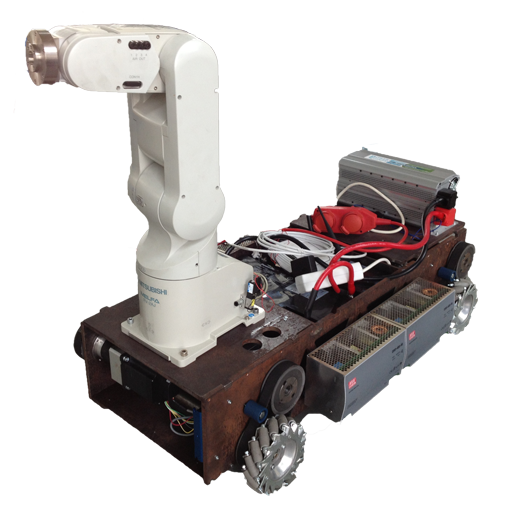
\includegraphics[width=.6\textwidth]{Abbildungen/Roboter} 
\caption[Mecanum-Roboter]{Mecanum-Roboter.}
\label{fig:Roboter}
\end{figure}

\section{Mecanum-Roboter}
\label{sec:Mecanum-Roboter}

Der Mecanum-Roboter ist 1000 mm lang und 610 mm breit. Er ist mit vier Mecanum-Rädern ausgestattet. Der Radstand beträgt 775 mm und die Spurbreite beträgt 490 mm. Die Räder haben einen Durchmesser von 115 mm und besitzen jeweils 15 Hilfsrollen.

Die Anordnung der Mecanum-Räder ermöglicht dem Mecanum-Roboter omnidirektionale Bewegungen.
Er kann sich ohne Verstellen der Räder in jede Richtung fortbewegen und auf der Stelle drehen.

\subsection*{Mecanum-Räder}
\label{sec:Mecanum-Raeder}
\begin{figure}
\centering
 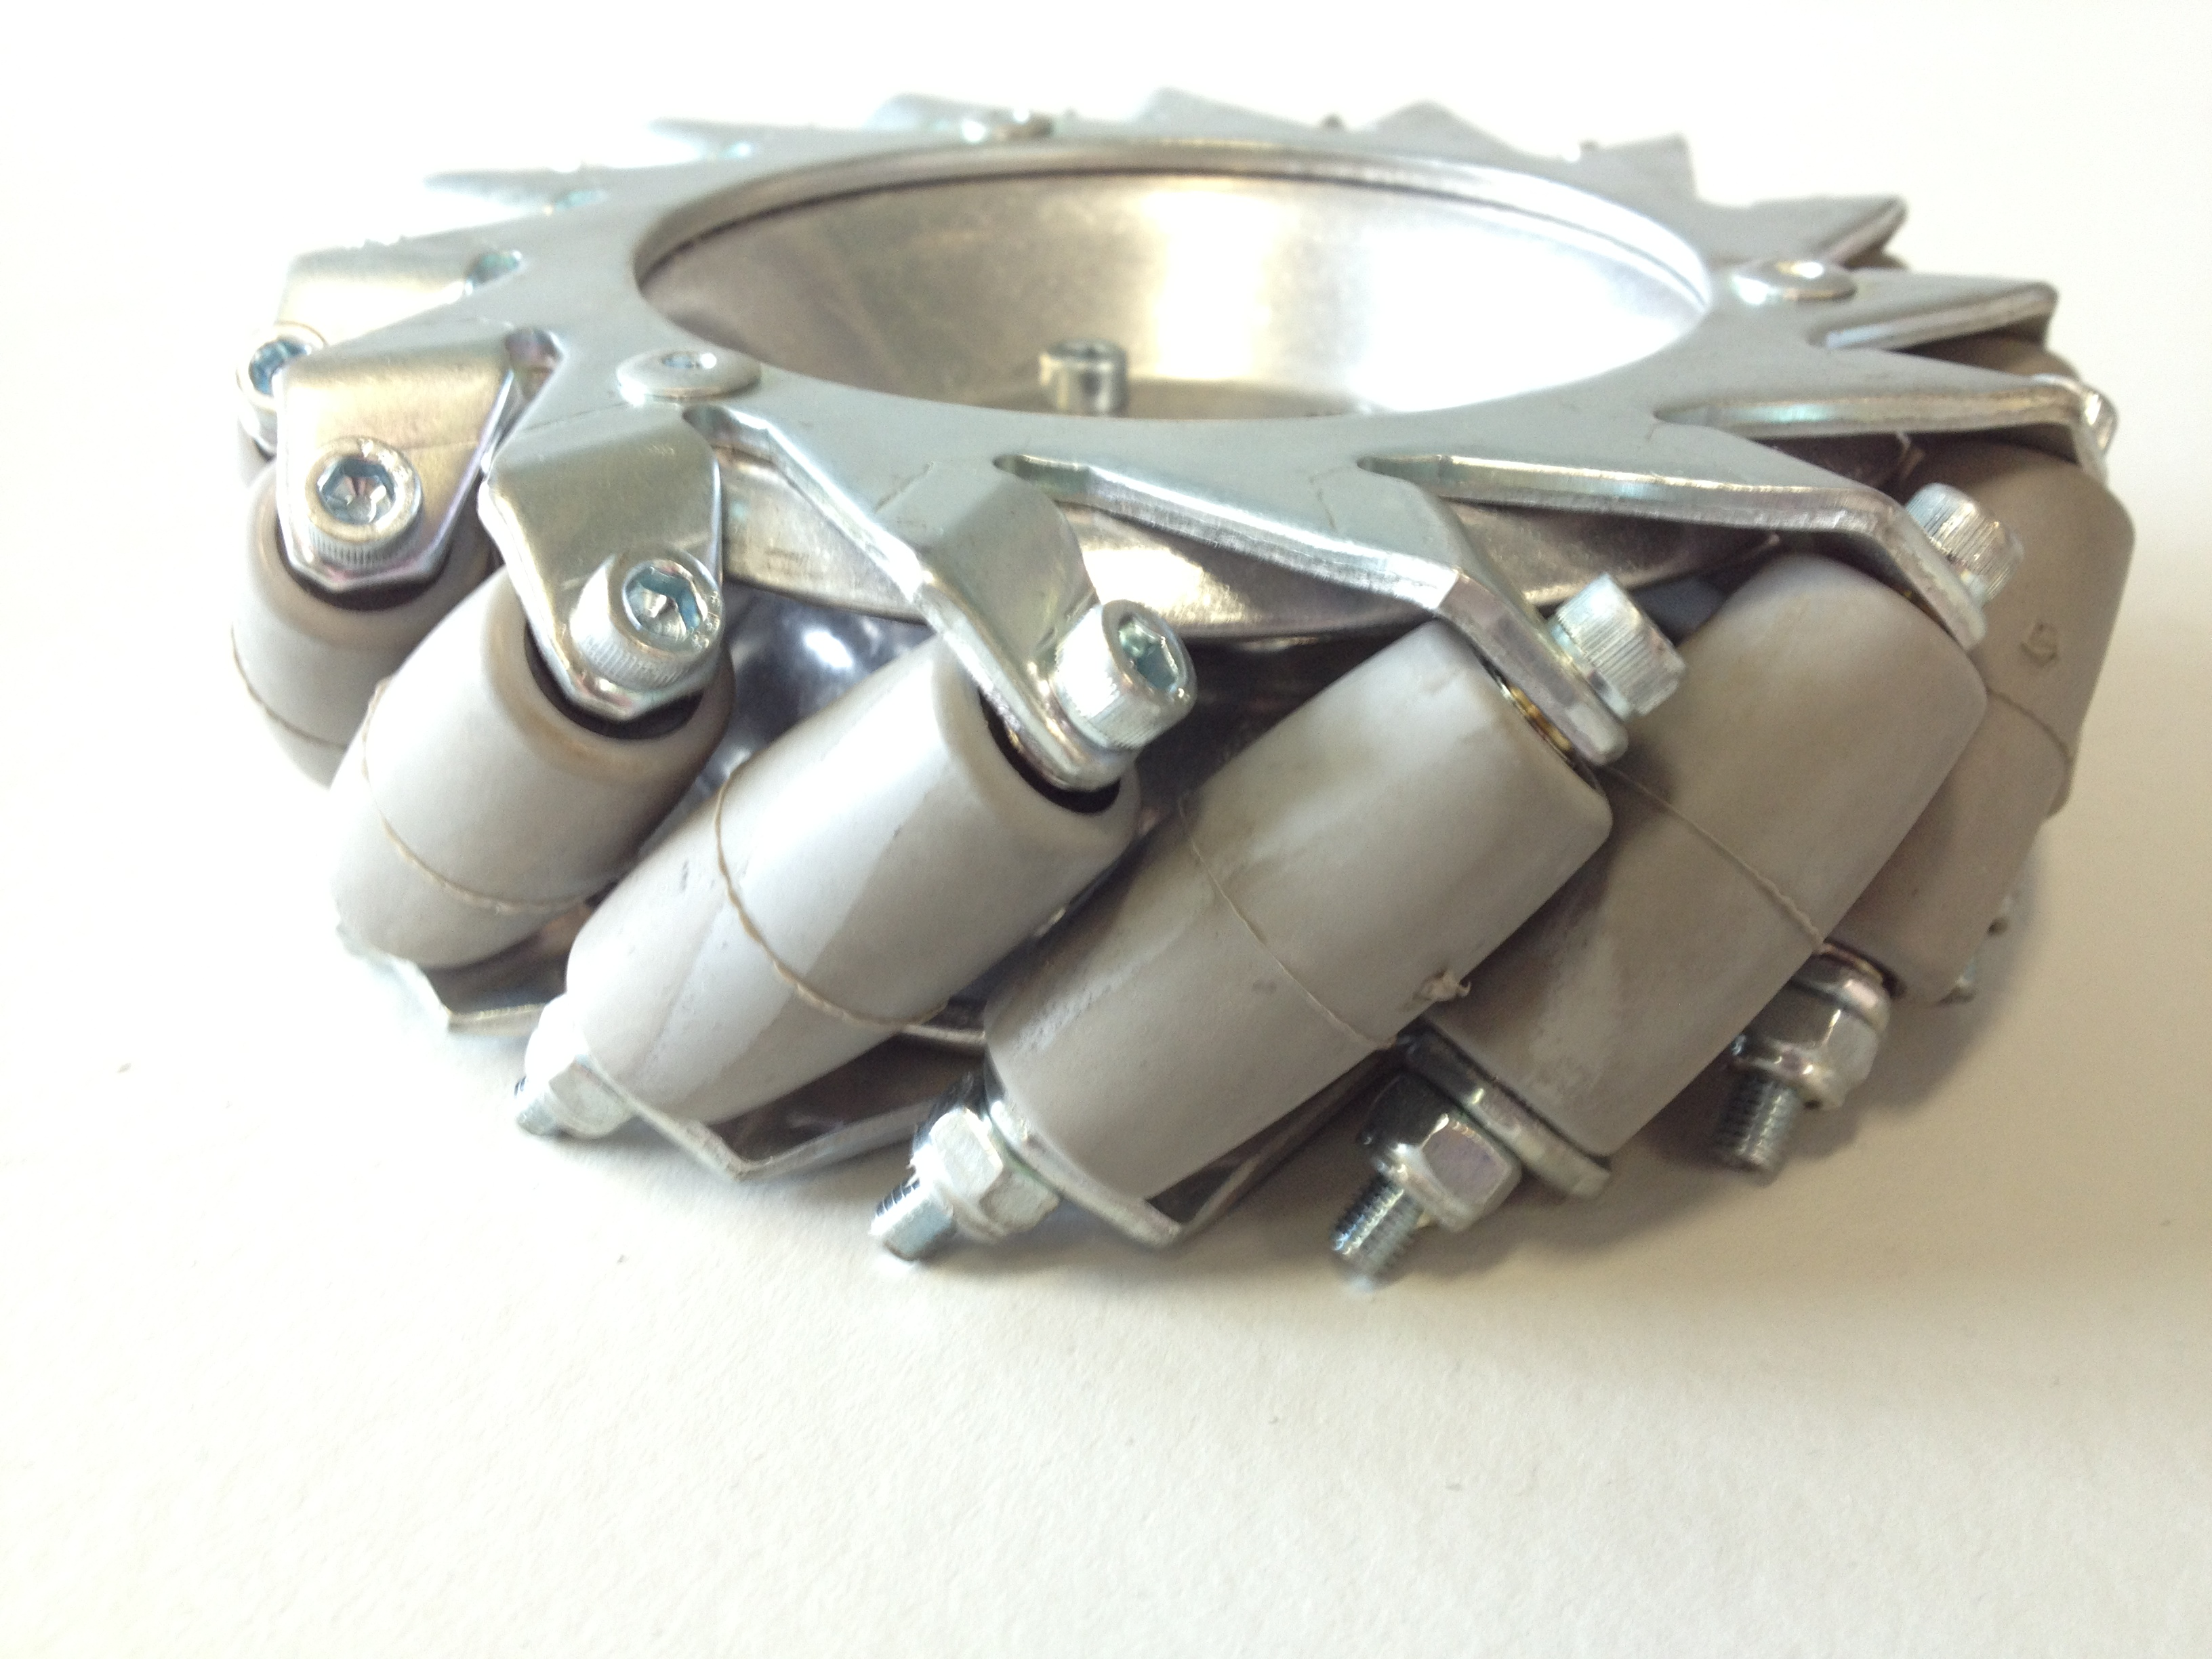
\includegraphics[width=.6\textwidth]{Abbildungen/Mecanumrad} 
\caption[Mecanum-Rad]{Ein Mecanum Rad mit tonnenförmigen Hilfsrädern}
\label{fig:Mecanum-Rad}
\end{figure}
Das Mecanum Rad wurde 1973 von der schwedischen Firma Mecanum AB entwickelt und bedient unterschiedliche Anwendungen. Heutige Anwendungsbeispiele sind unter anderem Förderfahrzeuge, fahrerlose Transportfahrzeuge oder Mobilitätshilfen. Auch in der Robotik finden die Allseitenräder immer häufiger Verwendung.
Abbilung \ref{fig:Mecanum-Rad} zeigt ein Mecanum-Rad des Mecanum-Roboters. Auf dem Umfang des Rades sind 15 tonnenförmige beschichtete Rollen im Winkel von 45 Grad zur Radachse angebracht. Diese Rollen haben keinen eigenen Antrieb und sind frei drehbar gelagert. Ausschließlich die Rollen haben Kontakt zum Boden.
Jedes Mecanum-Rad wird von einem Schrittmotor angetrieben. Somit sind Drehsinn und Drehzahl für jedes Rad einzeln ansteuerbar. Dieses ist entscheidend für die omnidirektionale Bewegung.
Durch eine individuelle Drehrichtungsauswahl entstehen durch die Hilfsrollen am Untergrund Kraftvektoren in unterschiedliche Richtungen. Die Summe der Vektoren aller Räder bildet die Gesamtbewegungsrichtung oder auch ein Gesamtdrehmoment.





















